%\documentclass[handout]{beamer}
\documentclass[ignorenonframetext]{beamer}
\usepackage{textpos}
\usepackage{graphicx}
\usepackage{pgf}
\usepackage{caption}
\usepackage{multimedia}
\usepackage{gensymb}
\usepackage{amsmath, mathrsfs}

\captionsetup[figure]{labelformat=empty}% redefines the caption setup of the figures environment in the beamer class.

\usetheme{Boadilla}
\usefonttheme{serif}
% \mode<presentation>
% {
%  \usefonttheme{serif}
% % \useoutertheme{sidebar}
% %   \logo{
\includegraphics[height=1cm]{elec_logo.pdf}}
% }

\title{TART Signal Correlators}

\author[Molteno, Suggate]{Tim Molteno, Pat Suggate}

\institute[Otago]
{
  Elec Research \\
  Department of Physics\\
  University of Otago \\
  Dunedin, New Zealand.\\
  tim@elec.ac.nz
}

% \titlegraphic{
\includegraphics[width=2cm]{fig/elec_logo.pdf}\hspace*{4.75cm}~%
%    
\includegraphics[width=2cm]{fig/elec_logo.pdf}
% }

\logo{\pgfputat{\pgfxy(-0.72,7.7)}{\pgfbox[center,base]{
\includegraphics[width=1cm]{./array_design/fig/elec_logo.pdf}}}} 

\date[ICEAA '19] % (optional, should be abbreviation of conference name)
{}

% \addtobeamertemplate{headline}{}{%
% \begin{textblock*}{100mm}(0.87\textwidth,2mm)
% 
\includegraphics[height=1.5cm]{elec_logo.pdf}
% \end{textblock*}}

\begin{document}


\begin{frame}
  \titlepage
\end{frame}

\begin{frame}{The radio signal}
Each radio receiver, say the one connected to antenna $a$, produces a complex number, $Z_a$ representing the voltage amplitude.
\[ Z_a = I_a + j Q_a \]

\begin{block}{Why complex numbers?}
They can be written as $Z_a = r_a e^{j \phi_a}$, where $r_a$ represents the scaling of the sinusoid, and $\phi_a$ is the phase of the sinusoid. So the single complex number represents both amplitude and phase.
\end{block}

These samples are generated by each radio 8 million times per second. There are 24 radios/antennas in a TART, so this means 196 million complex samples per second.
\end{frame}


% 
\begin{frame}{For each baseline}

A baseline exists for each pair of antennas.

For each sample from antennas $a$ and $b$
 \begin{eqnarray*}
  Z_a & = & I_a + j\,Q_a \\
  Z_b & = & I_b + j\,Q_b \\
  v_{ab} & = & Z_a \cdot Z_b^* = \mathcal{R}_{ab} + j \mathcal{I}_{ab} \\
  \mathcal{R}_{ab}  &  \equiv & I_a \cdot I_b + Q_a \cdot Q_b \\
  \mathcal{I}_{ab} & \equiv & Q_a \cdot I_b - I_a \cdot Q_b \
\end{eqnarray*}

$v_{ab}$ is the visibility of that single sample. This is also the {\em correlation}.
\end{frame}


\begin{frame}{Single-sample visibility calculation}
But TART data is single-bit binary. A value 1 represents +1, 0 represents -1.
\begin{center}
\begin{tabular}{llllllll}
$I_a$ & $Q_a$ & $I_b$ & $Q_b$ &  $\mathcal{R}_{ab}$ &    & $\mathcal{I}_{ab}$ &    \\
\hline
 0     & 0     & 0     & 0     &   0b010              & 2  & 0b000              & 0  \\
 0     & 0     & 0     & 1     &   0b000              & 0  & 0b010              & 2  \\
 0     & 0     & 1     & 0     &   0b000              & 0  & 0b110              & -2 \\
 0     & 0     & 1     & 1     &   0b110              & -2 & 0b000              & 0  \\
 0     & 1     & 0     & 0     &   0b000              & 0  & 0b110              & -2 \\
 0     & 1     & 0     & 1     &   0b010              & 2  & 0b000              & 0  \\
 0     & 1     & 1     & 0     &   0b110              & -2 & 0b000              & 0  \\
 0     & 1     & 1     & 1     &   0b000              & 0  & 0b010              & 2  
\end{tabular}
\end{center}
This calculation is just a look-up-table (LUT)
\end{frame}

\begin{frame}{FPGA}
 The TART does this for every pair of antennas, so it has 276 of these single-sample visibilities happening in parallel. This is done using a Field Programmable Gate Array (FPGA).
\centering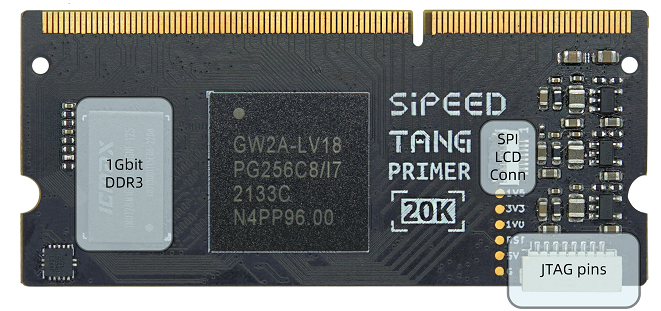
\includegraphics[width=0.7\linewidth]{20k_front.png}
 
 \url{https://wiki.sipeed.com/hardware/en/tang/tang-primer-20k/primer-20k.html}
\end{frame}


\begin{frame}{Snapshot Visibility}

Each visibility is the sum of the single-sample visibiities over an interval $T$, which consists of $N$ samples. 
\[ V_{ab} = \sum_{i=0}^{N} v_{ab} \]
This adding is also done by the FPGA..
\begin{itemize}
 \item The longer the interval, the lower the noise on the visibility
 \item If the data has lots of noise, the visibility will be close to zero.
\end{itemize}


\begin{block}{Remember}
 That is all that there is to it. Visibilities are simple sums of products.
\end{block}
\end{frame}

\end{document}
